\documentclass[11pt]{article}
\usepackage[margin=1in]{geometry}
\usepackage[T1]{fontenc}
\usepackage{lmodern}
\usepackage{xcolor}
\usepackage{graphicx}
\usepackage{amsmath,amssymb,amsthm}
\usepackage{algorithm}
\usepackage{algpseudocode}
\usepackage{booktabs}
\usepackage{multirow}
\usepackage{float}
\usepackage{subcaption}
\usepackage{tikz}
\usepackage{pgfplots}
\pgfplotsset{compat=1.17}
\usetikzlibrary{automata,positioning,arrows.meta}
\usepackage{hyperref}
\usepackage{cleveref}
% \usepackage[disable]{todonotes}
\usepackage{todonotes}

\theoremstyle{plain}
\newtheorem{theorem}{Theorem}
\newtheorem{lemma}[theorem]{Lemma}
\newtheorem{proposition}[theorem]{Proposition}
\newtheorem{corollary}[theorem]{Corollary}
\theoremstyle{definition}
\newtheorem{definition}{Definition}
\newtheorem{example}{Example}
\theoremstyle{remark}
\newtheorem{remark}{Remark}

\algrenewcommand{\algorithmicrequire}{\textbf{Input:}}
\algrenewcommand{\algorithmicensure}{\textbf{Output:}}

% Notation, kept in step with latex/main.tex so the two documents read alike.
\newcommand{\Ifree}{\mathcal{I}_{f}}
\newcommand{\Iknown}{\mathcal{I}_{k}}
\newcommand{\Ofree}{\mathcal{O}_{f}}
\newcommand{\Oknown}{\mathcal{O}_{k}}
\newcommand{\Tin}{T_{\mathit{Inp}}}
\newcommand{\Tout}{T_{\mathit{Out}}}
\newcommand{\psiin}{\psi_{\mathit{Inp}}}  % LTLf language of \Tin (assumption)
\newcommand{\psiout}{\psi_{\mathit{Out}}} % LTLf language of \Tout (guarantee)
\newcommand{\Sin}{S_{\mathit{Inp}}}
\newcommand{\Sout}{S_{\mathit{Out}}}
\newcommand{\cons}{\mathrm{cons}}
\newcommand{\mirror}[1]{\widetilde{#1}} % past-LTLf mirror of a future formula
\newcommand{\rev}[1]{#1^{\mathrm{R}}}   % reversal of a word / automaton / language
\newcommand{\Xdep}{\mathcal{X}}         % dependent output set
\newcommand{\Ydep}{\mathcal{Y}}         % set \Xdep is dependent on
\newcommand{\LTLf}{\text{LTL}_f}
\newcommand{\algname}[1]{\textbf{\textsc{#1}}}
\newcommand{\tool}[1]{\texttt{#1}}

% Review notes: one colour per author.
\newcommand{\na}[2][]{\todo[color=cyan,#1]{NA: {#2}}}
\newcommand{\cl}[2][]{\todo[color=green!30,#1]{CL: {#2}}}

% \guide{...}: what a section should hold. Delete each one once its section is written,
% or set \guidesfalse in main.tex to hide them all at once.
\newif\ifguides\guidestrue
\newcommand{\guide}[1]{\ifguides{\small\itshape\color{gray!70!black}[Guide: #1]}\fi}

% \guidesfalse % uncomment to hide every writing guide

\title{LTLf Synthesis with External Knowledge}
\author{Nadav Alon}
\date{\today}

\begin{document}
\maketitle

\begin{abstract}
Progress report on $\LTLf$ with external knowledge work. The problem is synthesis of an $\LTLf$ formula $\varphi$ assuming the possible traces are limited to those consistent with transducers $\Tin$ and $\Tout$, for input and output respectively. This idea was motivated by the TACAS'24 paper on output dependencies~\cite{AkshayBasaChakrabortyFried2024}; this generalizes the idea to input dependencies. The method we suggest uses MTDFA with on-the-fly formula progression and game solving, which hopefully prunes out enough paths that the original formula considers possible to outweigh the cost of the product.
In practice, trying to apply this to input transducers has mostly not paid off.
Against Spot's \tool{ltlfsynt} (full synthesis, median wall time at $N=6$ in the 2026-11-14 HPC sweep of \cref{sec:results}; speed-ups are \tool{ltlfsynt} time over \tool{otf-solve-simp}), \tool{otf-solve-simp} is ahead on every family with an \tool{ltlfsynt} time except slippery, from $2.56\times$ (hidden-counter) to $20.43\times$ (co-generated, where \tool{ltlfsynt} times out in one of the two cells) (\cref{fig:speedup}).
On the slippery family \tool{ltlfsynt} is slightly faster, at $0.88\times$ in aggregate; only the one-hot arm is ahead of it, at about $2\times$.
Knowledge itself buys little under the simplifier: knowledge against no knowledge is within $0.55$--$1.17\times$ on every family with a finite no-knowledge time, the exception being co-generated, where the no-knowledge side times out (\cref{tab:rq2}).
A comparison with output dependencies is difficult to make, as the output dependencies results~\cite{AkshayBasaChakrabortyFried2024} are for LTL and would need revising to compare.
\end{abstract}

\tableofcontents
\newpage

\section{Introduction}\label{sec:intro}

\subsection{Motivation}
\guide{Why $\LTLf$ synthesis matters (planning, robotics, business processes). Why classic
synthesis treats the environment as fully adversarial, and why that is often too pessimistic or
too expensive. One concrete scenario where something is \emph{known} about inputs or outputs.}
Reactive LTL synthesis is a problem in which we are given a specification $\varphi$ in Linear Temporal Logic (LTL) and we want to construct a controller that interacts with every environment such that the resulting trace satisfies the specification.

The TACAS'24 paper~\cite{AkshayBasaChakrabortyFried2024} introduced the ideas of variable dependencies in LTL synthesis, which allows us to classify some variables as dependent on others, and reduce the size of the problem. This result is restricted to output variables; attempting to apply the definition to input variables found none. This makes intuitive sense; the definition given in the paper is one that assumes control of the variable is the system's and not the environment, so formulas that do have such dependencies are likely to be valid and uninteresting, so they do not exist in benchmarks.

We wanted to generalize the idea of dependencies to input variables as well, and ended up with an even more general idea, in which we solve the synthesis problem with the help of an outside helper that decides the values of some variables.

\subsection{External Knowledge}

\guide{The idea in plain words: part of the inputs and/or outputs is governed by a known
component, given as a transducer. What this buys: realizability that would otherwise fail, and
smaller search spaces. Preview the running example.}

Given a specification $\varphi$, we want to be able to incorporate external knowledge about some variables. For that we model the knowledge as a transducer which according to the history of the other variables decides the values of the variables.
When solving the synthesis problem, we consult the transducer to determine the values of the variables it controls to limit the traces to the allowed ones.

This idea can be used to incorporate knowledge inherent to the formula itself (output dependencies) or to change the problem to a different one (similarly to fairness assumptions).

\subsection{Contributions}
\guide{Bullet list. Problem formulation; the five methods (NFA product, DFA product, three
on-the-fly variants); knowledge extraction from dependencies; implementation on Spot; benchmark
suite and results. Mark which items are done vs.\ in progress.}

\begin{itemize}
  \item Definitions of \begin{itemize}
    \item External knowledge
    \item $\LTLf$ synthesis with external knowledge
    \item $\LTLf$ synthesis with input dependencies
  \end{itemize}
  \item Several benchmark families to test the problem
  \item Implementation of methods to solve the problem, comparisons between them, and a comparison against the state of the art.
\end{itemize}

\section{Background}\label{sec:background}

\subsection{\texorpdfstring{$\LTLf$}{LTLf}}
\guide{Syntax and finite-trace semantics; strong/weak next ($X[!]$ vs.\ $X$); notation for
traces over $2^{\mathcal{I}\cup\mathcal{O}}$. Cite \cite{DeGiacomoVardi2013}.}

\subsection{Automata on Finite Words}
\guide{NFA, DFA, determinisation blow-up, minimisation. Past-$\LTLf$ and the reverse/mirror
construction that gives a small NFA (needed for Method 1).}

\subsection{Reactive Synthesis on Finite Traces}
\guide{Controller as a transducer; realizability; DFA game, attractor/fixpoint solving.
Turn order (who moves first). Cite \cite{PnueliRosner1989,DeGiacomoVardi2015}.}

\subsection{Symbolic Representations}
\guide{BDDs, multi-terminal DFAs (MTDFA) in Spot; why an mtdfa representation is a second
implementation of a method, not a new method. Cite \cite{Spot2022}.}

\subsection{Baseline Tool: \tool{ltlfsynt}}
\guide{What Spot's \tool{ltlfsynt} does, and how it is used here: as a baseline and as an
external realizability oracle.}

\section{Problem Definition}\label{sec:problem}

\subsection{Setting}
\guide{Variables $\mathcal{I}=\Ifree\cup\Iknown$, $\mathcal{O}=\Ofree\cup\Oknown$. Goal
$\varphi$. Who controls what.}

\subsection{Knowledge as Transducers}
\guide{Define $\Tin$ (states $\Sin$) and $\Tout$ (states $\Sout$), their input/output alphabets,
and the lambda split. Small figure of each.}

\begin{definition}[External-knowledge transducer]\label{def:ek-transducer}
\guide{formal definition}
\end{definition}

\subsection{Consistency}
\guide{When a trace agrees with $\Tin$, $\Tout$ and $T_C$; the $\cons$ predicate.}

\begin{definition}[Consistency]\label{def:consistency}
\guide{formal definition}
\end{definition}

\subsection{The Synthesis Problem}
\begin{definition}[Synthesis with external knowledge]\label{def:problem}
\guide{Given $(\varphi,\mathcal{I},\mathcal{O},\Tin,\Tout)$, find $T_C$ such that every consistent
trace satisfies $\varphi$, or report unrealizable.}
\end{definition}

\subsection{Running Example}
\begin{example}\label{ex:running}
\guide{One small instance used throughout: realizable with knowledge, unrealizable without.}
\end{example}

\subsection{Relation to Assume--Guarantee Synthesis}
\guide{When $\Tin$ has an $\LTLf$ language $\psiin$, the problem reduces to
$\psiin \rightarrow \varphi$ (and $\psiout$ as a guarantee). When it does not
(non-star-free $\Tin$), the reduction is unavailable. Introduce comparability tiers T1/T2/T3.}

\subsection{Complexity}
\guide{Known bounds, or what is open. Keep to what is proved.}

\section{Algorithms}\label{sec:algorithms}

\guide{Shared interface: every method takes $(\varphi,\mathcal{I},\mathcal{O},\Tin,\Tout)$ and returns
a controller or ``unrealizable''. State the common correctness claim once here.}

\subsection{Method 1: NFA Product}\label{sec:nfa}
\subsubsection{From \texorpdfstring{$\LTLf$}{LTLf} to a Small NFA}
\guide{Formula mirror, reversal; size theorem.}
\subsubsection{Product Construction}
\guide{Product of the Goal NFA with $\Tin$, $\Tout$; how consistency prunes.}
\subsubsection{Solving}
\guide{Subset/game construction on the product; extracting $T_C$.}
\subsubsection{Correctness and Complexity}
\guide{Theorem statement; proof sketch here, full proof in \cref{app:proofs}.}

\begin{algorithm}[H]
\caption{NFA product}\label{alg:nfa}
\begin{algorithmic}[1]
\Require $\varphi$, $\mathcal{I}$, $\mathcal{O}$, $\Tin$, $\Tout$
\Ensure controller $T_C$ or \textsc{Unrealizable}
\State \guide{pseudocode}
\end{algorithmic}
\end{algorithm}

\subsection{Method 2: DFA Product}\label{sec:dfa}
\subsubsection{Construction}
\guide{Full DFA for $\varphi$, product with the transducers, game solve.}
\subsubsection{Correctness and Complexity}
\guide{Theorem, proof sketch.}

\subsection{Method 3: On-the-Fly DFA Products}\label{sec:otf}
\guide{Why on-the-fly: build only the part of the product the game reaches.}
\subsubsection{Method 3.1: No Aggregation}
\guide{Construction; what is explored; early termination.}
\subsubsection{Method 3.2: Aggregation}
\guide{What is aggregated; soundness (implication, not equality, vs.\ the non-aggregating
methods). Status: not implemented.}
\subsubsection{Method 3.3: Dynamic Aggregation}
\guide{Construction; when it aggregates. Status: not implemented.}

\subsection{Explicit vs.\ Symbolic Representations}
\guide{Which methods exist in which representation (explicit, mtdfa, mtnfa). Table.}

\subsection{Comparison of the Methods}
\begin{table}[H]
\centering
\caption{Methods at a glance.}\label{tab:methods}
\begin{tabular}{llllll}
\toprule
Method & Goal automaton & Representation(s) & Worst-case size & Status \\
\midrule
1 NFA product      & & & & \\
2 DFA product      & & & & \\
3.1 OTF, no agg.   & & & & \\
3.2 OTF, agg.      & & & & \\
3.3 OTF, dyn.\ agg. & & & & \\
\bottomrule
\end{tabular}
\end{table}

\section{Extracting External Knowledge from Dependencies}\label{sec:dependencies}

\guide{Where do $\Tin$/$\Tout$ come from when the user does not supply them? Derive them from
dependencies already implied by $\varphi$.}

\subsection{Output Dependencies}
\begin{definition}[Output dependency]\label{def:outdep}
\guide{$\Xdep$ dependent on $\Ydep$.}
\end{definition}
\guide{Lemma: how a dependency yields a $\Tout$. Detection procedure.}

\subsection{Input Dependencies}
\begin{definition}[Input dependency]\label{def:indep}
\guide{formal definition}
\end{definition}
\guide{Lemma: how it yields a $\Tin$. Detection procedure.}

\subsection{Discussion}
\guide{How much knowledge these extractors find in practice; limitations; the ``tentative''
dependency generation tool.}

\section{Implementation}\label{sec:implementation}

\subsection{Architecture}
\guide{C++20 on Spot; thin wrappers; custom lambda-split transducer and NFA types; one
\texttt{Synthesis} interface. Diagram optional.}

\subsection{Tools}
\guide{\tool{ltlf-ek-synth} (CLI), \tool{ltlf-ek-bench} (benchmark runner), dependency tools.
Input formats (HOA transducers, formula files).}

\subsection{Verification Strategy}
\guide{The oracle layers: unit fixtures, cross-method equivalence, controller verifier, external
\tool{ltlfsynt} oracle. What each catches. Test-suite size.}

\subsection{Engineering Lessons}
\guide{Optional. Anything non-obvious that shaped the results (e.g.\ degenerate families,
timing vs.\ state counts).}

\section{Benchmarks}\label{sec:benchmarks}

\subsection{Research Questions}
\guide{What the experiments answer. E.g.\ RQ1: do the methods agree and verify? RQ2: how much does
knowledge shrink the product? RQ3: speed vs.\ \tool{ltlfsynt}? RQ4: which method wins where?}

\begin{enumerate}
  \item[RQ1] \guide{question}
  \item[RQ2] \guide{question}
\end{enumerate}

\subsection{Metrics}
\guide{Structural (state counts, deterministic, committed) vs.\ timing (wall clock, median of
repeats). Prune ratio; nk-product ratio; speedup. Why state counts are the decisive number.}

\subsection{Baselines}
\guide{\tool{ltlfsynt} on the $\psiin\rightarrow\varphi$ encoding; the no-knowledge product;
the unpruned product. Comparability tiers: which families admit a fair external comparison.}

\subsection{Benchmark Families}
\guide{One paragraph per family: $\varphi_n$, knowledge, tier, what it isolates. Then the
summary table.}

\subsubsection{Parametric Families}
\guide{cons-prunes, cons-inert, mirror-small, mirror-degenerate, parity-t3, knowledge-chain(-inert),
co-generated, \ldots}

\subsubsection{Engineered Domain Families}
\guide{Domain-inspired instances (e.g.\ slippery world, hidden counters).}

\subsubsection{External Suites}
Of the 430 instances with at most 16 propositions, 388 could be analysed and 6 of those carry output dependencies; a seventh, with 26 propositions, lies above that bound.

\subsubsection{Generated Corpus}
\guide{Random instances used for oracle soak testing.}

\begin{table}[H]
\centering
\caption{Benchmark families.}\label{tab:families}
\begin{tabular}{lllll}
\toprule
Family & $\varphi_n$ & Knowledge & Tier & Purpose \\
\midrule
 & & & & \\
\bottomrule
\end{tabular}
\end{table}

\subsection{Experimental Setup}
The timing sweep ran on the HPC cluster (nodes \texttt{cn01} and \texttt{cn16}, Intel Xeon Gold 6130 at 2.10\,GHz) from a Release build at commit \texttt{4e3beec} with Spot 2.15.1.
Each cell is repeated 5 times with a 20\,s timeout, for $n$ up to 6; the committed run is \texttt{docs/runs/2026-11-14-summary-paper-sweep.json}.
The RQ1 correctness checks ran on the developer's desktop, not on the HPC, and are machine-independent.
The SYNTCOMP verdict cross-checks come from the 2026-08-18 SYNTCOMP-fin sweep (\texttt{docs/runs/2026-08-18-syntcomp-fin-sweep.json}), run on the desktop with tools built at commit \texttt{40c5d72} and Spot 2.15.1.
The generated-corpus checks are oracle soaks with no committed run.
Repeats are aggregated by their median.

\section{Results}\label{sec:results}

\guide{One subsection per research question. Lead each with the claim, then the evidence.}

\subsection{Correctness: Agreement and Verification}
\guide{Cross-method agreement, controller verification, verdict mismatches vs.\ \tool{ltlfsynt}.}

\begin{table}[H]
\centering
\small
\begin{tabular}{lrrrrrr}
\toprule
family & dfa & nfa & mtdfa & mtnfa & otf-solve-simp & mismatches \\
\midrule
co-generated & 5.86 / 147.37 & 66.18 / t/o & 3.91 / 65.56 & 50.02 / t/o & 2.14 / t/o & 0 \\
cons-inert & 3.01 / 2.91 & 18.04 / 17.90 & 2.37 / 2.23 & 27.74 / 27.49 & 1.91 / 1.90 & 0 \\
cons-prunes & 3.28 / 2.52 & 14.40 / 12.64 & 3.07 / 2.72 & 16.60 / 12.75 & 2.34 / 2.16 & 0 \\
hidden-counter & 23.25 / 248.44 & 203.67 / 2332.03 & 7.11 / 14.49 & 171.80 / 14513.06 & 14.10 / 16.49 & 0 \\
knowledge-chain & 3.15 / n/a & 14.37 / n/a & 2.69 / n/a & 16.26 / n/a & 2.09 / n/a & 0 \\
knowledge-chain-inert & 7.28 / n/a & 170.59 / n/a & 3.21 / n/a & 95.68 / n/a & 4.02 / n/a & 0 \\
mirror-degenerate & 2.98 / 2.86 & 17.94 / 17.82 & 2.27 / 2.19 & 27.42 / 27.38 & 1.93 / 1.85 & 0 \\
mirror-small & 3.96 / 3.80 & 10.07 / 10.05 & 2.54 / 2.31 & 10.50 / 10.42 & 1.91 / 1.91 & 0 \\
slippery & 236.61 / 2263.08 & 90.75 / t/o & 343.60 / 674.51 & 1281.40 / t/o & 651.11 / 407.16 & 0 \\
\bottomrule
\end{tabular}

\caption{Median wall time in ms at the largest $N$, each variant with knowledge over without (\tool{-nk}); \tool{t/o} where no cell finished. The last column counts verdict mismatches against \tool{ltlfsynt}.}\label{tab:rq1}
\end{table}

\subsection{Effect of Knowledge on Product Size}
\guide{Prune ratio and nk-product ratio per family as $n$ grows. Figure.}

\begin{figure}[H]
\centering
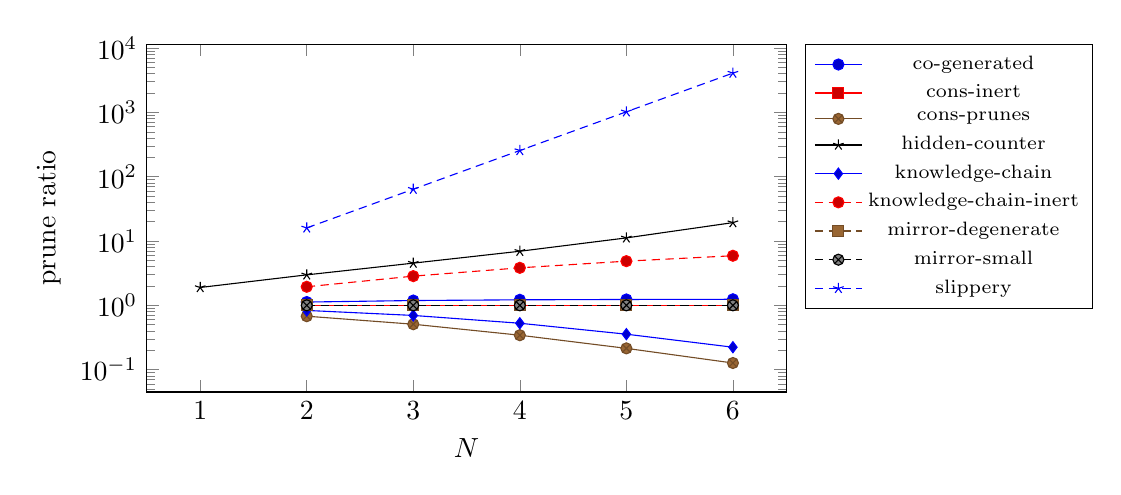
\begin{tikzpicture}
\begin{axis}[width=.8\linewidth, height=6cm, xlabel={$N$}, ylabel={prune ratio}, ymode=log, legend pos=outer north east, legend style={font=\scriptsize}]
\addplot coordinates {(2,1.125) (3,1.188) (4,1.219) (5,1.234) (6,1.242)};
\addlegendentry{co-generated}
\addplot coordinates {(2,1) (3,1) (4,1) (5,1) (6,1)};
\addlegendentry{cons-inert}
\addplot coordinates {(2,0.6778) (3,0.5085) (4,0.3431) (5,0.2142) (6,0.1268)};
\addlegendentry{cons-prunes}
\addplot coordinates {(1,1.896) (2,2.979) (3,4.533) (4,6.939) (5,11.19) (6,19.34)};
\addlegendentry{hidden-counter}
\addplot coordinates {(2,0.8333) (3,0.6966) (4,0.5266) (5,0.3559) (6,0.2232)};
\addlegendentry{knowledge-chain}
\addplot coordinates {(2,1.944) (3,2.846) (4,3.833) (5,4.865) (6,5.906)};
\addlegendentry{knowledge-chain-inert}
\addplot coordinates {(2,1) (3,1) (4,1) (5,1) (6,1)};
\addlegendentry{mirror-degenerate}
\addplot coordinates {(2,1) (3,1) (4,1) (5,1) (6,1)};
\addlegendentry{mirror-small}
\addplot coordinates {(2,16) (3,64) (4,256) (5,1024) (6,4096)};
\addlegendentry{slippery}

\end{axis}
\end{tikzpicture}
\caption{Reachable product states with knowledge over without, per family.}\label{fig:prune}
\end{figure}

\subsection{Runtime against \tool{ltlfsynt}}
\guide{Speedup per family; where \tool{ltlfsynt} times out. Figure + table.}

\begin{figure}[H]
\centering
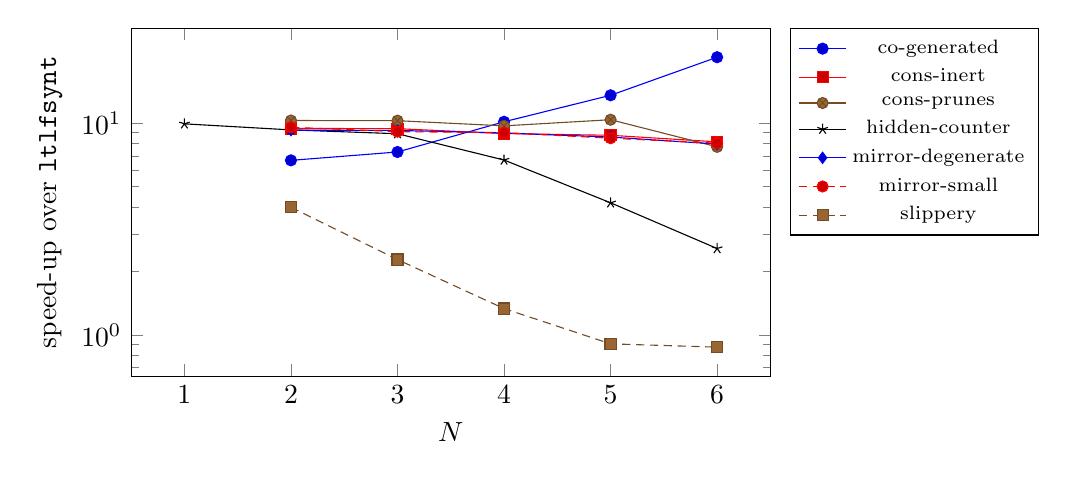
\begin{tikzpicture}
\begin{axis}[width=.8\linewidth, height=6cm, xlabel={$N$}, ylabel={speed-up over \tool{ltlfsynt}}, ymode=log, legend pos=outer north east, legend style={font=\scriptsize}]
\addplot coordinates {(2,6.662) (3,7.297) (4,10.13) (5,13.51) (6,20.43)};
\addlegendentry{co-generated}
\addplot coordinates {(2,9.424) (3,9.399) (4,8.915) (5,8.746) (6,8.145)};
\addlegendentry{cons-inert}
\addplot coordinates {(2,10.27) (3,10.25) (4,9.692) (5,10.36) (6,7.715)};
\addlegendentry{cons-prunes}
\addplot coordinates {(1,9.905) (2,9.275) (3,8.897) (4,6.685) (5,4.201) (6,2.556)};
\addlegendentry{hidden-counter}
\addplot coordinates {(2,9.247) (3,9.222) (4,8.968) (5,8.579) (6,7.953)};
\addlegendentry{mirror-degenerate}
\addplot coordinates {(2,9.543) (3,9.103) (4,9.002) (5,8.474) (6,8.027)};
\addlegendentry{mirror-small}
\addplot coordinates {(2,3.999) (3,2.267) (4,1.331) (5,0.9073) (6,0.8753)};
\addlegendentry{slippery}

\end{axis}
\end{tikzpicture}
\caption{\tool{ltlfsynt} full synthesis over \tool{otf-solve-simp}, median wall time per family.}\label{fig:speedup}
\end{figure}

\begin{table}[H]
\centering
% generated by python3 scripts/summary_paper_tables.py docs/runs/2026-11-14-summary-paper-sweep.json summary-paper/tables; do not edit
\begin{tabular}{lrrrrrr}
\toprule
family & $N$ & knowledge (ms) & no knowledge (ms) & knowledge speed-up & \tool{ltlfsynt} (ms) & \tool{ltlfsynt} stages (ms) \\
\midrule
co-generated & 6 & 2.14 & t/o & $\ge$ 9331.30$\times$ & 44.48 & 2.14 \\
cons-inert & 6 & 1.91 & 1.90 & 1.00$\times$ & 14.95 & 1.66 \\
cons-prunes & 6 & 2.34 & 2.16 & 0.92$\times$ & 18.08 & 2.19 \\
hidden-counter & 6 & 14.10 & 16.49 & 1.17$\times$ & 34.94 & 15.66 \\
knowledge-chain & 6 & 2.09 & n/a & n/a & n/a & n/a \\
knowledge-chain-inert & 6 & 4.02 & n/a & n/a & n/a & n/a \\
mirror-degenerate & 6 & 1.93 & 1.85 & 0.96$\times$ & 14.78 & 1.65 \\
mirror-small & 6 & 1.91 & 1.91 & 0.99$\times$ & 14.76 & 1.67 \\
slippery-binary & 6 & 614.34 & 337.47 & 0.55$\times$ & 462.31 & 243.22 \\
slippery-binary-compact & 6 & 628.73 & 402.54 & 0.64$\times$ & 385.12 & 257.23 \\
slippery-onehot & 6 & 4640.22 & 5237.96 & 1.13$\times$ & 9190.18 & 7715.97 \\
\bottomrule
\end{tabular}

\caption{Knowledge against no knowledge (\tool{otf-solve-simp} against \tool{nk-otfsolve-simp}), with \tool{ltlfsynt} as full synthesis and the sum of its internal stage times.}\label{tab:rq2}
\end{table}

\subsection{Comparison Between Methods}
\guide{Which method wins on which family, and why (NFA vs.\ DFA vs.\ on-the-fly; explicit vs.\
mtdfa).}

\subsection{Where Time Goes}
\guide{Stage breakdown: automaton construction, product, game solving. The on-the-fly
game-solving gap.}

\subsection{Negative and Surprising Results}
\guide{Degenerate families, non-reproductions, cases with no gain. Keep them; they are findings.}

\subsection{Threats to Validity}
\guide{Family selection bias, small $n$, timeouts, the tier assumptions, single machine.}

\section{Related Work}\label{sec:related}

\subsection{\texorpdfstring{$\LTLf$}{LTLf} Synthesis}
\guide{Classic and symbolic approaches; tools (\tool{ltlfsynt}, Lydia, Syft, Nike, \ldots).}

\subsection{Synthesis under Assumptions}
\guide{Assume--guarantee, environment specifications, GR(1)-style assumptions.}

\subsection{Partial Information and Knowledge}
\guide{Synthesis with incomplete information; plan/strategy with known components.}

\subsection{Positioning}
\guide{What this work does that the above do not.}

\section{Where We Are Headed}\label{sec:future}

\subsection{Current Status}
\guide{Done / partial / not started, per method and per tool. A short table works.}

\subsection{Open Theoretical Questions}
\guide{Unproved claims, gaps between \texttt{main.tex} and the implementation, expressibility
questions.}

\subsection{Algorithmic Next Steps}
\guide{Methods 3.2 and 3.3; better game solving on the fly; synthesising the dependencies.}

\subsection{Benchmarking Next Steps}
\guide{New families, larger $n$, more external instances.}

\subsection{Publication Plan}
\guide{Target venue(s), deadline(s), what must be done first.}

\subsection{Timeline}
\guide{Milestones by month.}

\subsection{Questions for the Advisor}
\guide{Decisions you need input on.}

\section{Conclusion}\label{sec:conclusion}
\guide{One paragraph: problem, approach, main result, next step.}


\bibliographystyle{plain}
\bibliography{refs}

\appendix
\section{Proofs}\label{app:proofs}
\guide{Full proofs for the theorems sketched in \cref{sec:algorithms,sec:dependencies}.}

\section{Full Results}\label{app:results}
\guide{Complete per-family tables. Put generated tables under \texttt{tables/} and
\texttt{\textbackslash input} them here.}

\section{Reproducibility}\label{app:repro}
\guide{Build commands, exact sweep invocations, commit hashes, where the run reports live
(\texttt{docs/runs/}).}


\end{document}
